\chapter{Windows development}

In the previous chapters, we delved into the world of eBPF and explored its versatile capabilities within the Linux ecosystem.
But eBPF is now a cross-platform technology: we are going to continue our journey beyond the confines of Linux to explain the possibilities of eBPF development on the Windows operating system. 
This chapter serves as a guide for developers and enthusiasts that want to utilize the power of eBPF for Windows-centric applications.

While eBPF is natively integrated into the Linux kernel, recent advancements have extended its reach to the Windows platform, making it accessible to a broader audience. 
This development opens up new horizons for network monitoring, security and performance analysis within Windows environments.

Since May 2021, Microsoft has been working on bringing eBPF to Windows. 
In fact, in recent times there have been significant developments in the integration of eBPF on the this platform. 
As of the time of writing this thesis in September 2023, eBPF for Windows is in a state of rapid evolution and expansion. 
In this chapter we’ll be looking at setting up a Windows-eBPF build environment, followed by developing, running and debugging eBPF programs on Windows, providing insights into its current status and potential future directions. 

Unlike what we saw for linux, to date there is only one way to work with eBPF on Windows: it involves using the \textit{ebpf-for-windows} open-source GitHub project by Microsoft \cite{eBPFWinGitHubRepo}.
This repository is full of documents that describe how to to get started and use eBPF on Windows.
We will make several references to these documents to avoid making the reading too heavy, but we will highlight the crucial passages.
To start working with ebpf on Windows, in fact, the experience is not as user-friendly as it was on Linux where it was enough to clone a repository.
This statement is not intended to discourage anyone, but it will immediately be clear that not so much the coding part as the setup of an environment will be very long and complex.

Moreover, we are going to present another project, called \textit{windows-ebpf-starter}, that was created to make the experience of eBPF programming within the Windows ecosystem easier \cite{WineBPFStarterRepo}: the result is that this project is for Windows what libbpf-bootstrap is for Linux.
However, at the time of writing, the parallelism is not true in every aspect: we are going to present later some issues that we came across while developing eBPF applications.

\section{Creation of the work environment}

In the previous chapter mentioned the fact that we needed a Linux environment in which we could develop various programs: to do so, we used VirtualBox.
Now we have to create another environment, this time for Windows, as we will study the state of the art of eBPF on this latest operating system. 

Remembering that the computer on which the process was carried out has Windows 11 as its operating system, for this purpose we used the \textit{Hyper-V Console Manager}, a native Windows feature, to create a separate Windows 11 virtual machine.
\textit{Hyper-V} is a type 1 (or bare-metal) virtualization software, also known as a \textit{Virtual Machine Monitor} (\textit{VMM}), which runs directly on the physical hardware without the need for an underlying host operating system. 
The illustrative representation of the architecture just described is depicted in Figure \ref{fig:type_1_hypervisor}.
As the core software responsible for managing virtual machines and allocating hardware resources to each VM, Hyper-V ensures better security and resource utilization by isolating each VM from others and the host OS. 
With direct access to the physical hardware, it efficiently allocates resources, resulting in improved performance, isolation and scalability compared to type 2 hypervisors like VirtualBox.

\begin{figure}[h]
	\centering
	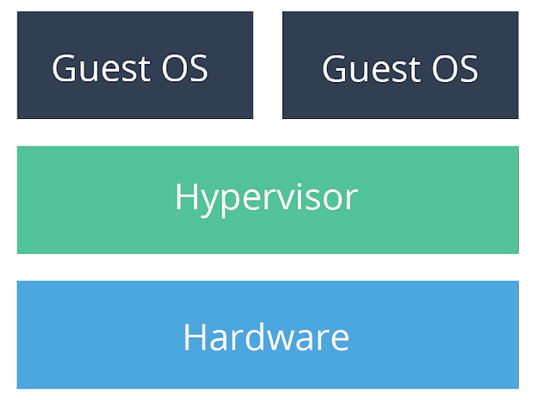
\includegraphics[width=0.7\linewidth]{images/Technologies/type_1_hypervisor.png}
	\caption{Type 1 (or bare metal) hypervisor architecture \cite{HypervisorsArchitectures}.}
	\label{fig:type_1_hypervisor}
\end{figure}

The greatest benefits of hypervisors are their robustness and scalability, enabling the efficient virtualization of large-scale applications and services.
However, the choice of creating a virtual machine using the Hyper-V Console Manager was dictated by two other reasons:

\begin{itemize}
	\item 
		The setup instructions described on the ebpf-for-windows GitHub repository tell the user to install a Windows VM \cite{VMSetup};
	\item 
		The so created isolated Windows 11 development environment provided a controlled space for testing and optimizing eBPF programs on the Windows platform.
		In fact, if anything goes wrong in this environment, we can just delete the virtual machine and create a new one, while if something bad happens on our host machine, we could break our computer.
\end{itemize}

We are going to talk about the eBPF installation on Windows later: for now, besides the fact that that he virtual machine was configured with adequate resources to support development tasks effectively, the only thing worth noting is that during the quick creation of the virtual machine the option of ``Windows 11 dev environment'' must be selected (the tutorial tells to choose the ``Windows 10 dev environment'', but Windows 11 works as well).  


\section{ebpf for Windows}

% https://microsoft.github.io/ebpf-for-windows/ -> MANUAL PAGE

% https://github.com/Microsoft/ebpf-for-windows/ 

\section{windows ebpf starter}

% https://github.com/SubconsciousCompute/windows-ebpf-starter